\documentclass[12pt,aspectratio=169]{beamer}
\usepackage[T1]{fontenc}
\usepackage{lmodern,amsmath,amssymb,booktabs,tikz,graphicx}
\usetikzlibrary{arrows.meta,positioning,calc}
\definecolor{Ink}{HTML}{17324D}
\definecolor{Teal}{HTML}{007F7A}
\definecolor{Muted}{HTML}{556574}
\definecolor{Paper}{HTML}{FAFAF7}
\definecolor{Rust}{HTML}{AD532E}
\definecolor{Gold}{HTML}{B38630}
\setbeamercolor{background canvas}{bg=Paper}
\setbeamercolor{normal text}{fg=Ink}
\setbeamercolor{frametitle}{fg=Ink}
\setbeamercolor{structure}{fg=Teal}
\setbeamercolor{alerted text}{fg=Rust}
\setbeamerfont{frametitle}{size=\LARGE,series=\bfseries}
\setbeamertemplate{navigation symbols}{}
\setbeamersize{text margin left=9mm,text margin right=9mm}
\setbeamertemplate{frametitle}{\par\vspace{2mm}\insertframetitle\par\vspace{1mm}{\color{Gold}\rule{14mm}{1pt}}}
\setbeamertemplate{footline}{\hspace{9mm}\scriptsize\color{Muted}\insertsectionhead\hfill\insertframenumber\hspace{9mm}\vspace{4mm}}
\hypersetup{colorlinks=true,urlcolor=Teal,linkcolor=Muted,pdfauthor={}}
\newcommand{\point}[1]{\par\vspace{3mm}{\large #1\par}}
\newcommand{\eqnote}[1]{\par\vspace{2mm}{\small\color{Muted}#1\par}}
\newcommand{\smalltext}[1]{\eqnote{#1}}
\newcommand{\insight}[1]{\par\vspace{2mm}{\color{Teal}\bfseries #1}\par}
\newcommand{\identity}{\text{\scriptsize accounting identity}}
\newcommand{\policy}{R^{\mathrm{policy}}}
\newcommand{\loanrate}{R^{\mathrm{loan}}}
\newcommand{\nominal}{R^{\mathrm{nom}}}
\newcommand{\realrate}{R^{\mathrm{real}}}
\newcommand{\neutral}{R^{\mathrm{neutral}}}
\newcommand{\spot}[1]{R^{\mathrm{spot}}(#1)}
\newcommand{\forward}[2]{R^{\mathrm{forward}}(#1,#2)}
\newcommand{\bondyield}{R^{\mathrm{bond}}}
\newcommand{\bondrate}[1]{R^{\mathrm{bond}}(#1)}
\AtBeginDocument{\setlength{\abovedisplayskip}{5pt}\setlength{\belowdisplayskip}{5pt}\setlength{\abovedisplayshortskip}{3pt}\setlength{\belowdisplayshortskip}{3pt}}

\hypersetup{pdftitle={Economics and Finance for Mathematicians: Output, income and capital flows}}
\begin{document}

% Slide 1: Output, income and capital flows

\begin{frame}[plain]
{\color{Teal}\large ECONOMICS AND FINANCE\quad /\quad 01}\par\vspace{9mm}{\Huge\bfseries Output, income and capital flows}\par\vspace{7mm}{\Large How do real resources become income, saving and financial claims?}
\end{frame}

% Slide 2: The seven-class route

\begin{frame}{The seven-class route}
\begin{center}\begin{tabular}{@{}p{.43\textwidth}p{.51\textwidth}@{}}\toprule \textbf{Class} & \textbf{Question}\\\midrule 1. Accounting and flows & Who produces, spends and finances?\\[2mm]
2. Money, inflation and activity & How does policy affect demand?\\[2mm]
3. Bonds and yield curves & How are future payments priced?\\[2mm]
4. Foreign exchange & How are currencies priced?\\[2mm]
5. Open-economy policy & Which adjustment is possible?\\[2mm]
6. Crises and the euro & How does financial fragility spread?\\[2mm]
7. Debt and macro trades & How do fiscal and market risks interact?\\\bottomrule\end{tabular}\end{center}
\end{frame}

% Slide 3: Production and income
\section[Production and income]{Production and income}
\begin{frame}[plain]
{\color{Gold}\large LECTURE 1}\par\vspace{9mm}{\Huge\bfseries Production and income}\par\vspace{7mm}{\Large Why can we measure the same economy in three ways?}
\end{frame}

% Slide 4: A loaf of bread

\begin{frame}{A loaf of bread}
\begin{center}
\includegraphics[trim=0bp 110bp 0bp 150bp,clip,width=.93\textwidth,height=4.2cm,keepaspectratio]{assets/bakery.png}\end{center}\eqnote{Invented bakery economy. The farmer, mill and bakery each add value.}
\end{frame}

% Slide 5: Value added along the chain

\begin{frame}{Value added along the chain}
\begin{center}\begin{tabular}{@{}llll@{}}\toprule \textbf{Producer} & \textbf{Sales} & \textbf{Bought inputs} & \textbf{Value added}\\\midrule Farmer & 10 & 0 & 10\\[2mm]
Mill & 25 & 10 & 15\\[2mm]
Bakery & 60 & 25 & 35\\[2mm]
Total &  &  & 60\\\bottomrule\end{tabular}\end{center}\eqnote{One period, one currency, no taxes or imports. Bread is the final good.}
\end{frame}

% Slide 6: Output generates income

\begin{frame}{Output generates income}
\begin{center}\begin{tabular}{@{}llll@{}}\toprule \textbf{Producer} & \textbf{Wages} & \textbf{Operating surplus} & \textbf{Value added}\\\midrule Farmer & 6 & 4 & 10\\[2mm]
Mill & 10 & 5 & 15\\[2mm]
Bakery & 25 & 10 & 35\\[2mm]
Total & 41 & 19 & 60\\\bottomrule\end{tabular}\end{center}\eqnote{Each unit of value added accrues to labour or the business owners.}
\end{frame}

% Slide 7: Three measurements of one flow

\begin{frame}{Three measurements of one flow}
\begin{center}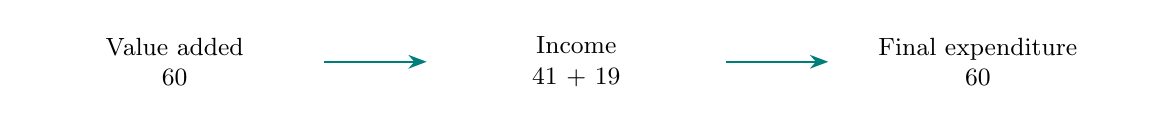
\begin{tikzpicture}[>=Stealth,every node/.style={font=\small,align=center,text width=3.5cm}]\node at (0.0,0){Value added\\60};\node at (5.1,0){Income\\41 + 19};\node at (10.2,0){Final expenditure\\60};\draw[->,Teal,thick] (1.9,0)--(3.1999999999999997,0);\draw[->,Teal,thick] (7.0,0)--(8.299999999999999,0);\end{tikzpicture}\end{center}\point{Production, income and expenditure count the same activity.}
\end{frame}

% Slide 8: GDP counts current domestic production

\begin{frame}{GDP counts current domestic production}
\point{Final goods and services produced inside the economy.}\point{Investment includes new capital and changes in inventories.}\point{Purchases of existing shares or old houses are asset trades.}
\end{frame}

% Slide 9: Nominal output and real output

\begin{frame}{Nominal output and real output}
\[GDP^{\rm nominal}_t=Q_tY_t.\]\point{$Y_t$: real output. $Q_t$: the GDP price deflator.}\point{Nominal growth combines more production and higher prices.}
\end{frame}

% Slide 10: Growth rates separate prices and quantities

\begin{frame}{Growth rates separate prices and quantities}
\[1+g_{\rm nominal}=(1+g_{\rm real})(1+\pi_{\rm GDP}).\]\[1.03\times1.02-1=5.06\%.\]\eqnote{Hypothetical 3\% real growth and 2\% GDP-deflator inflation.}
\end{frame}

% Slide 11: Accounting and equilibrium
\section[Accounting and equilibrium]{Accounting and equilibrium}
\begin{frame}[plain]
{\color{Gold}\large LECTURE 1}\par\vspace{9mm}{\Huge\bfseries Accounting and equilibrium}\par\vspace{7mm}{\Large Which equalities always hold, and which need a model?}
\end{frame}

% Slide 12: Expenditure in a closed economy

\begin{frame}{Expenditure in a closed economy}
\[\boxed{Y=C+I+G.}\]\point{$C$: private consumption. $I$: gross domestic investment.}\point{$G$: government purchases. No international trade yet.}
\end{frame}

% Slide 13: Unsold bread still has an accounting destination

\begin{frame}{Unsold bread still has an accounting destination}
\[Y=60,\qquad C=50,\qquad I_{\rm inventory}=10.\]\point{Production is 60. Customers spend 50.}\point{The bakery holds 10 of newly produced unsold bread.}
\end{frame}

% Slide 14: Equilibrium adds planned spending

\begin{frame}{Equilibrium adds planned spending}
\[Y=C^{\rm plan}+I^{\rm plan}+G.\]\begin{center}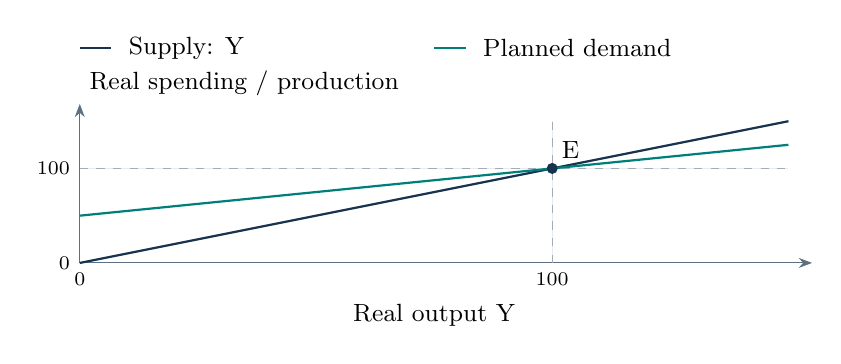
\begin{tikzpicture}[>=Stealth,every node/.style={font=\small}]
\draw[Ink!10] (0.0000,0.0000)--(0.0000,1.8000);\node[below,font=\scriptsize] at (0.0000,0.0000){0};
\draw[Ink!10] (6.0000,0.0000)--(6.0000,1.8000);\node[below,font=\scriptsize] at (6.0000,0.0000){100};
\draw[Ink!10] (0.0000,0.0000)--(9.0000,0.0000);\node[left,font=\scriptsize] at (0.0000,0.0000){0};
\draw[Ink!10] (0.0000,1.2000)--(9.0000,1.2000);\node[left,font=\scriptsize] at (0.0000,1.2000){100};
\draw[->,Ink!70] (0,0)--(9.3,0);\draw[->,Ink!70] (0,0)--(0,2.02);
\node[below] at (4.5,-.40){Real output Y};\node[anchor=west] at (0,2.2800000000000002){Real spending / production};
\draw[Ink!40,dashed] (0.0000,1.2000)--(9.0000,1.2000);
\draw[Ink!40,dashed] (6.0000,0.0000)--(6.0000,1.8000);
\draw[Ink,thick] plot coordinates {(0.0000,0.0000) (9.0000,1.8000)};
\draw[Teal,thick] plot coordinates {(0.0000,0.6000) (9.0000,1.5000)};
\fill[Ink] (6.0000,1.2000) circle (2pt);\node[above right] at (6.0000,1.2000){E};
\draw[Ink,thick] (0.0,2.73)--(0.4,2.73);\node[anchor=west,font=\small] at (0.5,2.73){Supply: Y};
\draw[Teal,thick] (4.5,2.73)--(4.9,2.73);\node[anchor=west,font=\small] at (5.0,2.73){Planned demand};
\end{tikzpicture}\end{center}\eqnote{At E, planned spending equals output. Prices are fixed in this model.}
\end{frame}

% Slide 15: Potential output and the long run

\begin{frame}{Potential output and the long run}
\[\boxed{Y^*=A K^\alpha(L^*)^{1-\alpha},\qquad0<\alpha<1.}\]\point{$A$: productivity. $K$: capital. $L^*$: labour at normal employment.}\point{$\alpha$: output elasticity of capital in this Cobb--Douglas model.}\eqnote{Potential is sustainable output. The long-run benchmark has $Y=Y^*$.}
\end{frame}

% Slide 16: The output gap connects activity to rates

\begin{frame}{The output gap connects activity to rates}
\[\text{Output gap}=100\,\frac{Y-Y^*}{Y^*}.\]\[Y=95,\quad Y^*=100\quad\Rightarrow\quad\text{gap}=-5\%.\]\point{Below potential: spare capacity can reduce inflation pressure.}\point{Above potential: stretched resources can increase inflation pressure.}\eqnote{This helps interpret central-bank decisions. The next plot shows a gap closing.}
\end{frame}

% Slide 17: A recession can be an equilibrium with slack

\begin{frame}{A recession can be an equilibrium with slack}
\begin{center}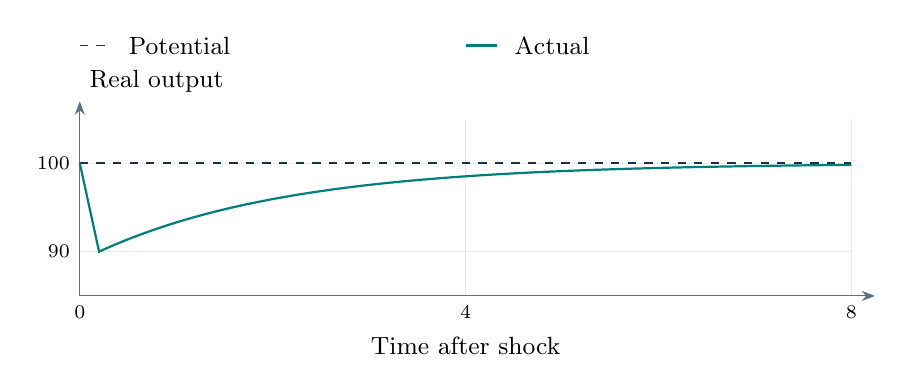
\begin{tikzpicture}[>=Stealth,every node/.style={font=\small}]
\draw[Ink!10] (0.0000,0.0000)--(0.0000,2.2500);\node[below,font=\scriptsize] at (0.0000,0.0000){0};
\draw[Ink!10] (4.9000,0.0000)--(4.9000,2.2500);\node[below,font=\scriptsize] at (4.9000,0.0000){4};
\draw[Ink!10] (9.8000,0.0000)--(9.8000,2.2500);\node[below,font=\scriptsize] at (9.8000,0.0000){8};
\draw[Ink!10] (0.0000,0.5625)--(9.8000,0.5625);\node[left,font=\scriptsize] at (0.0000,0.5625){90};
\draw[Ink!10] (0.0000,1.6875)--(9.8000,1.6875);\node[left,font=\scriptsize] at (0.0000,1.6875){100};
\draw[->,Ink!70] (0,0)--(10.100000000000001,0);\draw[->,Ink!70] (0,0)--(0,2.47);
\node[below] at (4.9,-.40){Time after shock};\node[anchor=west] at (0,2.73){Real output};
\draw[Ink,dashed,thick] plot coordinates {(0.0000,1.6875) (9.8000,1.6875)};
\draw[Teal,thick] plot coordinates {(0.0000,1.6875) (0.2450,0.5625) (0.3675,0.6174) (0.4900,0.6696) (0.6125,0.7192) (0.7350,0.7664) (0.8575,0.8113) (0.9800,0.8541) (1.1025,0.8947) (1.2250,0.9334) (1.3475,0.9702) (1.4700,1.0052) (1.5925,1.0384) (1.7150,1.0701) (1.8375,1.1002) (1.9600,1.1288) (2.0825,1.1561) (2.2050,1.1820) (2.3275,1.2067) (2.4500,1.2301) (2.5725,1.2524) (2.6950,1.2736) (2.8175,1.2938) (2.9400,1.3130) (3.0625,1.3313) (3.1850,1.3487) (3.3075,1.3652) (3.4300,1.3809) (3.5525,1.3959) (3.6750,1.4101) (3.7975,1.4236) (3.9200,1.4365) (4.0425,1.4487) (4.1650,1.4604) (4.2875,1.4714) (4.4100,1.4820) (4.5325,1.4920) (4.6550,1.5015) (4.7775,1.5106) (4.9000,1.5192) (5.0225,1.5274) (5.1450,1.5352) (5.2675,1.5427) (5.3900,1.5497) (5.5125,1.5565) (5.6350,1.5628) (5.7575,1.5689) (5.8800,1.5747) (6.0025,1.5802) (6.1250,1.5854) (6.2475,1.5904) (6.3700,1.5952) (6.4925,1.5997) (6.6150,1.6039) (6.7375,1.6080) (6.8600,1.6119) (6.9825,1.6156) (7.1050,1.6191) (7.2275,1.6224) (7.3500,1.6256) (7.4725,1.6286) (7.5950,1.6315) (7.7175,1.6342) (7.8400,1.6368) (7.9625,1.6393) (8.0850,1.6416) (8.2075,1.6439) (8.3300,1.6460) (8.4525,1.6480) (8.5750,1.6500) (8.6975,1.6518) (8.8200,1.6535) (8.9425,1.6552) (9.0650,1.6568) (9.1875,1.6583) (9.3100,1.6597) (9.4325,1.6610) (9.5550,1.6623) (9.6775,1.6636) (9.8000,1.6647)};
\draw[Ink,dashed] (0.0,3.18)--(0.4,3.18);\node[anchor=west,font=\small] at (0.5,3.18){Potential};
\draw[Teal,thick] (4.9,3.18)--(5.300000000000001,3.18);\node[anchor=west,font=\small] at (5.4,3.18){Actual};
\end{tikzpicture}\end{center}\eqnote{Hypothetical demand shock. The closing gap is a modelled adjustment.}
\end{frame}

% Slide 18: Saving and investment in a closed economy

\begin{frame}{Saving and investment in a closed economy}
\[S\equiv Y-C-G.\]\[Y=C+I+G\quad\Rightarrow\quad \boxed{S=I.}\]\point{Saving is income not consumed by households or government.}
\end{frame}

% Slide 19: Private and public saving

\begin{frame}{Private and public saving}
\[S_p=Y-T-C,\qquad S_g=T-G.\]\[S=S_p+S_g.\]\point{$T$: taxes less current transfers.}\point{A public deficit may be matched by private saving or investment changes.}
\end{frame}

% Slide 20: The rest of the world
\section[The rest of the world]{The rest of the world}
\begin{frame}[plain]
{\color{Gold}\large LECTURE 1}\par\vspace{9mm}{\Huge\bfseries The rest of the world}\par\vspace{7mm}{\Large How do trade, investment income and transfers connect?}
\end{frame}

% Slide 21: Domestic expenditure and trade

\begin{frame}{Domestic expenditure and trade}
\[\boxed{Y=C+I+G+X-M.}\]\point{$X$: exports. $M$: imports. $NX\equiv X-M$.}\point{Imports are removed because spending categories include foreign output.}
\end{frame}

% Slide 22: An imported machine

\begin{frame}{An imported machine}
\[\Delta I=10,\qquad\Delta M=10.\]\[\Delta Y=\Delta I-\Delta M=0.\]\point{No extra domestic production at the purchase date in this stripped-down example.}
\end{frame}

% Slide 23: From domestic production to residents’ income

\begin{frame}{From domestic production to residents’ income}
\[GNI=Y+NPI.\]\point{$NPI$: net primary income received from abroad.}\point{Think interest, dividends, reinvested earnings and cross-border labour income.}
\end{frame}

% Slide 24: Primary income: an ownership example

\begin{frame}{Primary income: an ownership example}
\begin{center}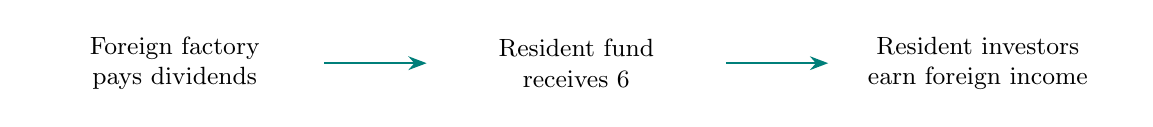
\begin{tikzpicture}[>=Stealth,every node/.style={font=\small,align=center,text width=3.5cm}]\node at (0.0,0){Foreign factory\\pays dividends};\node at (5.1,0){Resident fund\\receives 6};\node at (10.2,0){Resident investors\\earn foreign income};\draw[->,Teal,thick] (1.9,0)--(3.1999999999999997,0);\draw[->,Teal,thick] (7.0,0)--(8.299999999999999,0);\end{tikzpicture}\end{center}\[\text{Income received }6-\text{income paid abroad }2=NPI=4.\]\eqnote{Invented resident/nonresident transactions, in one currency.}
\end{frame}

% Slide 25: Current transfers add disposable income

\begin{frame}{Current transfers add disposable income}
\[GNDI=Y+NPI+NSI.\]\point{$NSI$: net secondary income from abroad.}\point{A resident abroad sending a family remittance is a concrete example.}
\end{frame}

% Slide 26: The current account is our net current flow from abroad

\begin{frame}{The current account is our net current flow from abroad}
\point{It adds what residents receive from the rest of the world, less what they pay, for trade, income and current transfers.}\[\boxed{CA=(X-M)+NPI+NSI.}\]\point{A deficit means current payments exceed receipts. The gap needs external financing.}\eqnote{This is why the current account connects trade to saving, investment and funding needs.}
\end{frame}

% Slide 27: Saving finances investment at home or abroad

\begin{frame}{Saving finances investment at home or abroad}
\[S\equiv GNDI-C-G.\]\[GNDI=C+I+G+CA.\]\[\boxed{S-I=CA.}\]
\end{frame}

% Slide 28: A deficit can finance productive investment

\begin{frame}{A deficit can finance productive investment}
\begin{center}\begin{tabular}{@{}llll@{}}\toprule \textbf{Economy} & \textbf{Saving} & \textbf{Investment} & \textbf{CA}\\\midrule New investment opportunity & 20 & 30 & -10\\[2mm]
High consumption, same saving gap & 10 & 20 & -10\\\bottomrule\end{tabular}\end{center}\point{The same current-account deficit can reflect different economic stories.}
\end{frame}

% Slide 29: US borrowing and dollar privilege
\section[US borrowing and dollar privilege]{US borrowing and dollar privilege}
\begin{frame}[plain]
{\color{Gold}\large LECTURE 1}\par\vspace{9mm}{\Huge\bfseries US borrowing and dollar privilege}\par\vspace{7mm}{\Large Why does the world keep financing the United States?}
\end{frame}

% Slide 30: The financial counterpart

\begin{frame}{The financial counterpart}
\[CA+KA=FA\quad\text{when measured without errors}.\]\point{$KA$: capital-account balance.}\point{$FA$: net acquisition of foreign assets minus net incurrence of liabilities.}
\end{frame}

% Slide 31: Foreign investors help finance US spending

\begin{frame}{Foreign investors help finance US spending}
\begin{center}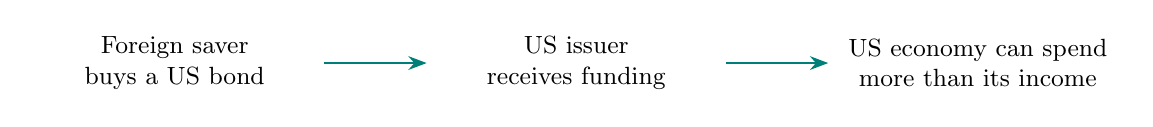
\begin{tikzpicture}[>=Stealth,every node/.style={font=\small,align=center,text width=3.5cm}]\node at (0.0,0){Foreign saver\\buys a US bond};\node at (5.1,0){US issuer\\receives funding};\node at (10.2,0){US economy can spend\\more than its income};\draw[->,Teal,thick] (1.9,0)--(3.1999999999999997,0);\draw[->,Teal,thick] (7.0,0)--(8.299999999999999,0);\end{tikzpicture}\end{center}\[CA_{\rm US}=-\$246.0\text{ billion in Q2 2026}.\]\eqnote{BEA, release 24 September 2026. The diagram illustrates one financing channel.}
\end{frame}

% Slide 32: Net international investment position

\begin{frame}{Net international investment position}
\[\boxed{NIIP=\text{assets held abroad}-\text{foreign claims on us}.}\]\point{The current account is a flow over a period. NIIP is a balance sheet at a date.}\point{A negative NIIP means foreign claims exceed residents’ foreign assets.}\eqnote{Claims include equity and direct investment as well as debt.}
\end{frame}

% Slide 33: The US external balance sheet is large on both sides

\begin{frame}{The US external balance sheet is large on both sides}
\begin{center}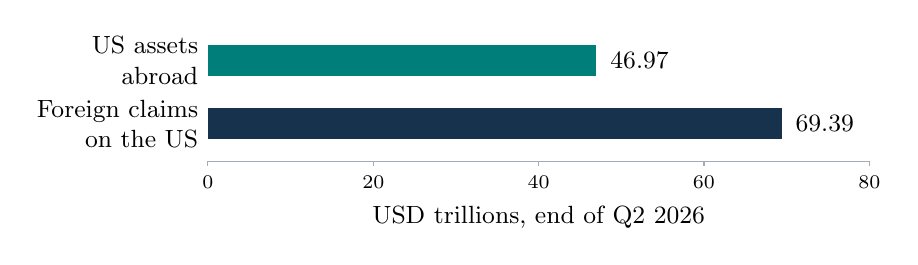
\begin{tikzpicture}[x=.105cm,y=.8cm,every node/.style={font=\small}]
\node[anchor=east,align=right] at (0,.25){US assets\\abroad};
\node[anchor=east,align=right] at (0,-.75){Foreign claims\\on the US};
\fill[Teal] (0,0) rectangle (46.97,.5);
\fill[Ink] (0,-1) rectangle (69.39,-.5);
\node[anchor=west] at (47.5,.25){46.97};
\node[anchor=west] at (69.9,-.75){69.39};
\draw[Ink!40] (0,-1.35)--(80,-1.35);
\foreach \v in {0,20,40,60,80}{\draw[Ink!40](\v,-1.35)--(\v,-1.43);\node[below,font=\scriptsize]at(\v,-1.43){\v};}
\node[below]at(40,-1.9){USD trillions, end of Q2 2026};
\end{tikzpicture}\end{center}\[NIIP=46.97-69.39=-\$22.42\text{ trillion}.\]\eqnote{BEA, end of Q2 2026. These positions include corporate equity and direct investment.}
\end{frame}

% Slide 34: What is the US “exorbitant privilege”?

\begin{frame}{What is the US “exorbitant privilege”?}
\point{Investors want dollar assets for reserves, payments and collateral.}\point{They may accept a lower yield for those services, reducing US funding costs.}\point{The US can borrow in dollars while owning riskier businesses abroad.}\eqnote{Dollar funding advantages and returns on the foreign portfolio both matter.}
\end{frame}

% Slide 35: Negative NIIP can coexist with positive investment income

\begin{frame}{Negative NIIP can coexist with positive investment income}
\begin{center}\begin{tabular}{@{}llll@{}}\toprule \textbf{Hypothetical external portfolio} & \textbf{Position} & \textbf{Income yield} & \textbf{Annual income}\\\midrule Foreign assets owned & 100 & 6\% & +6\\[2mm]
Liabilities to foreigners & 150 & 2\% & -3\\\bottomrule\end{tabular}\end{center}\[NIIP=100-150=-50,\qquad\text{net investment income}=6-3=+3.\]\eqnote{Illustrative income yields, excluding capital gains. These are not current US observations.}
\end{frame}

% Slide 36: US asset demand connects yields and the dollar

\begin{frame}{US asset demand connects yields and the dollar}
\begin{center}\begin{tabular}{@{}p{.44\textwidth}p{.49\textwidth}@{}}\toprule \textbf{Conditional change} & \textbf{Other inputs fixed}\\\midrule Fewer Treasury buyers & Lower prices, higher yields\\[2mm]
Less demand for dollar assets & Pressure on the dollar\\[2mm]
A weaker dollar & Higher dollar value of unhedged foreign assets\\\bottomrule\end{tabular}\end{center}\eqnote{These are conditional mechanisms. NIIP alone gives no market forecast.}
\end{frame}

% Slide 37: Risk sharing is a gain from international finance

\begin{frame}{Risk sharing is a gain from international finance}
\begin{center}\begin{tabular}{@{}lll@{}}\toprule \textbf{Two equally likely states} & \textbf{Home harvest} & \textbf{Foreign harvest}\\\midrule State A & 120 & 80\\[2mm]
State B & 80 & 120\\\bottomrule\end{tabular}\end{center}\point{Half-ownership of each harvest pays 100 in either state.}
\end{frame}

% Slide 38: Diversification depends on correlation

\begin{frame}{Diversification depends on correlation}
\begin{center}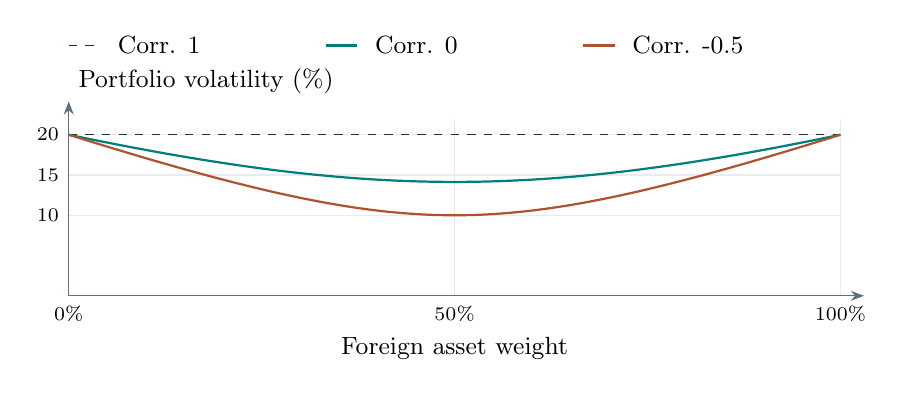
\begin{tikzpicture}[>=Stealth,every node/.style={font=\small}]
\draw[Ink!10] (0.0000,0.0000)--(0.0000,2.2500);\node[below,font=\scriptsize] at (0.0000,0.0000){0\%};
\draw[Ink!10] (4.9000,0.0000)--(4.9000,2.2500);\node[below,font=\scriptsize] at (4.9000,0.0000){50\%};
\draw[Ink!10] (9.8000,0.0000)--(9.8000,2.2500);\node[below,font=\scriptsize] at (9.8000,0.0000){100\%};
\draw[Ink!10] (0.0000,1.0227)--(9.8000,1.0227);\node[left,font=\scriptsize] at (0.0000,1.0227){10};
\draw[Ink!10] (0.0000,1.5341)--(9.8000,1.5341);\node[left,font=\scriptsize] at (0.0000,1.5341){15};
\draw[Ink!10] (0.0000,2.0455)--(9.8000,2.0455);\node[left,font=\scriptsize] at (0.0000,2.0455){20};
\draw[->,Ink!70] (0,0)--(10.100000000000001,0);\draw[->,Ink!70] (0,0)--(0,2.47);
\node[below] at (4.9,-.40){Foreign asset weight};\node[anchor=west] at (0,2.73){Portfolio volatility (\%)};
\draw[Ink,dashed] plot coordinates {(0.0000,2.0455) (0.0980,2.0455) (0.1960,2.0455) (0.2940,2.0455) (0.3920,2.0455) (0.4900,2.0455) (0.5880,2.0455) (0.6860,2.0455) (0.7840,2.0455) (0.8820,2.0455) (0.9800,2.0455) (1.0780,2.0455) (1.1760,2.0455) (1.2740,2.0455) (1.3720,2.0455) (1.4700,2.0455) (1.5680,2.0455) (1.6660,2.0455) (1.7640,2.0455) (1.8620,2.0455) (1.9600,2.0455) (2.0580,2.0455) (2.1560,2.0455) (2.2540,2.0455) (2.3520,2.0455) (2.4500,2.0455) (2.5480,2.0455) (2.6460,2.0455) (2.7440,2.0455) (2.8420,2.0455) (2.9400,2.0455) (3.0380,2.0455) (3.1360,2.0455) (3.2340,2.0455) (3.3320,2.0455) (3.4300,2.0455) (3.5280,2.0455) (3.6260,2.0455) (3.7240,2.0455) (3.8220,2.0455) (3.9200,2.0455) (4.0180,2.0455) (4.1160,2.0455) (4.2140,2.0455) (4.3120,2.0455) (4.4100,2.0455) (4.5080,2.0455) (4.6060,2.0455) (4.7040,2.0455) (4.8020,2.0455) (4.9000,2.0455) (4.9980,2.0455) (5.0960,2.0455) (5.1940,2.0455) (5.2920,2.0455) (5.3900,2.0455) (5.4880,2.0455) (5.5860,2.0455) (5.6840,2.0455) (5.7820,2.0455) (5.8800,2.0455) (5.9780,2.0455) (6.0760,2.0455) (6.1740,2.0455) (6.2720,2.0455) (6.3700,2.0455) (6.4680,2.0455) (6.5660,2.0455) (6.6640,2.0455) (6.7620,2.0455) (6.8600,2.0455) (6.9580,2.0455) (7.0560,2.0455) (7.1540,2.0455) (7.2520,2.0455) (7.3500,2.0455) (7.4480,2.0455) (7.5460,2.0455) (7.6440,2.0455) (7.7420,2.0455) (7.8400,2.0455) (7.9380,2.0455) (8.0360,2.0455) (8.1340,2.0455) (8.2320,2.0455) (8.3300,2.0455) (8.4280,2.0455) (8.5260,2.0455) (8.6240,2.0455) (8.7220,2.0455) (8.8200,2.0455) (8.9180,2.0455) (9.0160,2.0455) (9.1140,2.0455) (9.2120,2.0455) (9.3100,2.0455) (9.4080,2.0455) (9.5060,2.0455) (9.6040,2.0455) (9.7020,2.0455) (9.8000,2.0455)};
\draw[Teal,thick] plot coordinates {(0.0000,2.0455) (0.0980,2.0251) (0.1960,2.0050) (0.2940,1.9850) (0.3920,1.9653) (0.4900,1.9459) (0.5880,1.9266) (0.6860,1.9077) (0.7840,1.8889) (0.8820,1.8704) (0.9800,1.8522) (1.0780,1.8343) (1.1760,1.8167) (1.2740,1.7993) (1.3720,1.7822) (1.4700,1.7655) (1.5680,1.7491) (1.6660,1.7330) (1.7640,1.7172) (1.8620,1.7018) (1.9600,1.6867) (2.0580,1.6720) (2.1560,1.6577) (2.2540,1.6438) (2.3520,1.6302) (2.4500,1.6171) (2.5480,1.6043) (2.6460,1.5920) (2.7440,1.5802) (2.8420,1.5687) (2.9400,1.5578) (3.0380,1.5473) (3.1360,1.5372) (3.2340,1.5277) (3.3320,1.5186) (3.4300,1.5100) (3.5280,1.5020) (3.6260,1.4944) (3.7240,1.4874) (3.8220,1.4809) (3.9200,1.4750) (4.0180,1.4696) (4.1160,1.4648) (4.2140,1.4605) (4.3120,1.4567) (4.4100,1.4536) (4.5080,1.4510) (4.6060,1.4490) (4.7040,1.4475) (4.8020,1.4466) (4.9000,1.4464) (4.9980,1.4466) (5.0960,1.4475) (5.1940,1.4490) (5.2920,1.4510) (5.3900,1.4536) (5.4880,1.4567) (5.5860,1.4605) (5.6840,1.4648) (5.7820,1.4696) (5.8800,1.4750) (5.9780,1.4809) (6.0760,1.4874) (6.1740,1.4944) (6.2720,1.5020) (6.3700,1.5100) (6.4680,1.5186) (6.5660,1.5277) (6.6640,1.5372) (6.7620,1.5473) (6.8600,1.5578) (6.9580,1.5687) (7.0560,1.5802) (7.1540,1.5920) (7.2520,1.6043) (7.3500,1.6171) (7.4480,1.6302) (7.5460,1.6438) (7.6440,1.6577) (7.7420,1.6720) (7.8400,1.6867) (7.9380,1.7018) (8.0360,1.7172) (8.1340,1.7330) (8.2320,1.7491) (8.3300,1.7655) (8.4280,1.7822) (8.5260,1.7993) (8.6240,1.8167) (8.7220,1.8343) (8.8200,1.8522) (8.9180,1.8704) (9.0160,1.8889) (9.1140,1.9077) (9.2120,1.9266) (9.3100,1.9459) (9.4080,1.9653) (9.5060,1.9850) (9.6040,2.0050) (9.7020,2.0251) (9.8000,2.0455)};
\draw[Rust,thick] plot coordinates {(0.0000,2.0455) (0.0980,2.0149) (0.1960,1.9844) (0.2940,1.9541) (0.3920,1.9240) (0.4900,1.8941) (0.5880,1.8644) (0.6860,1.8349) (0.7840,1.8056) (0.8820,1.7765) (0.9800,1.7476) (1.0780,1.7190) (1.1760,1.6907) (1.2740,1.6626) (1.3720,1.6348) (1.4700,1.6073) (1.5680,1.5802) (1.6660,1.5533) (1.7640,1.5268) (1.8620,1.5007) (1.9600,1.4750) (2.0580,1.4497) (2.1560,1.4248) (2.2540,1.4004) (2.3520,1.3764) (2.4500,1.3529) (2.5480,1.3300) (2.6460,1.3077) (2.7440,1.2859) (2.8420,1.2647) (2.9400,1.2442) (3.0380,1.2244) (3.1360,1.2053) (3.2340,1.1869) (3.3320,1.1693) (3.4300,1.1526) (3.5280,1.1367) (3.6260,1.1216) (3.7240,1.1076) (3.8220,1.0945) (3.9200,1.0824) (4.0180,1.0713) (4.1160,1.0613) (4.2140,1.0524) (4.3120,1.0446) (4.4100,1.0380) (4.5080,1.0325) (4.6060,1.0282) (4.7040,1.0252) (4.8020,1.0233) (4.9000,1.0227) (4.9980,1.0233) (5.0960,1.0252) (5.1940,1.0282) (5.2920,1.0325) (5.3900,1.0380) (5.4880,1.0446) (5.5860,1.0524) (5.6840,1.0613) (5.7820,1.0713) (5.8800,1.0824) (5.9780,1.0945) (6.0760,1.1076) (6.1740,1.1216) (6.2720,1.1367) (6.3700,1.1526) (6.4680,1.1693) (6.5660,1.1869) (6.6640,1.2053) (6.7620,1.2244) (6.8600,1.2442) (6.9580,1.2647) (7.0560,1.2859) (7.1540,1.3077) (7.2520,1.3300) (7.3500,1.3529) (7.4480,1.3764) (7.5460,1.4004) (7.6440,1.4248) (7.7420,1.4497) (7.8400,1.4750) (7.9380,1.5007) (8.0360,1.5268) (8.1340,1.5533) (8.2320,1.5802) (8.3300,1.6073) (8.4280,1.6348) (8.5260,1.6626) (8.6240,1.6907) (8.7220,1.7190) (8.8200,1.7476) (8.9180,1.7765) (9.0160,1.8056) (9.1140,1.8349) (9.2120,1.8644) (9.3100,1.8941) (9.4080,1.9240) (9.5060,1.9541) (9.6040,1.9844) (9.7020,2.0149) (9.8000,2.0455)};
\draw[Ink,dashed] (0.0,3.18)--(0.4,3.18);\node[anchor=west,font=\small] at (0.5,3.18){Corr. 1};
\draw[Teal,thick] (3.266666666666667,3.18)--(3.666666666666667,3.18);\node[anchor=west,font=\small] at (3.766666666666667,3.18){Corr. 0};
\draw[Rust,thick] (6.533333333333334,3.18)--(6.9333333333333345,3.18);\node[anchor=west,font=\small] at (7.033333333333334,3.18){Corr. -0.5};
\end{tikzpicture}\end{center}\eqnote{Equal standalone volatility of 20\%. Hypothetical assets and correlations.}
\end{frame}

% Slide 39: What a macro release can and cannot tell a trader

\begin{frame}{What a macro release can and cannot tell a trader}
\point{GDP describes production relative to expectations and capacity.}\point{The current account describes net external funding needs.}\point{The US example shows why asset demand, income yields and portfolio risk matter.}
\end{frame}

% Slide 40: Counterfactual exercise: extra public consumption

\begin{frame}{Counterfactual exercise: extra public consumption}
\point{Government consumption rises by 2\% of GDP.}\point{Taxes, disposable income and investment initially stay fixed.}\point{Predict the change in national saving and the current account.}
\end{frame}

% Slide 41: The accounting answer and the economic question

\begin{frame}{The accounting answer and the economic question}
\[\Delta S=-2\%,\qquad\Delta CA=-2\%\text{ of GDP}.\]\point{If output or private saving responds, those numbers change.}\point{Next lecture supplies a model of demand and rates.}
\end{frame}

% Slide 42: Further reading
\section[Reading]{Reading}
\begin{frame}{Further reading}
\point{Dmitriy Sergeyev, Bocconi 30054 course materials.}\point{Krugman, Obstfeld \& Melitz, \emph{International Economics}.}\point{Source links and worked answers accompany each slide in the notes.}
\end{frame}
\end{document}
